\vssub
\subsection{~谱分区} \label{sub:num_part}
\conthead{APL Wave / XWaves / IMEDS}{B. Tracy, C. Bunney}

数值波浪模式预报的海况往往很复杂，这是因为其中同时存在由局地风作用和更远处风暴形成的多个波列。为更好地描述这些局地风海和远程涌浪分量，而不必处理模式波谱的全部复杂性，可将谱分割为若干谱格集合，并由这些集合推导出更易识别的波浪统计量（高度、周期、方向）。

\noindent
图~\ref{fig:partitions} 给出了某一网格点在特定时刻的能量密度谱表面图示例。该表面显示了每个频率-方向交点处的能量密度大小。表面被划分为若干阴影区域或分区，表示谱内子峰的能量。图~\ref{fig:partitions} 显示了四个谱分区：一个风海区和三个涌浪波列。该谱所代表的总能量可用有效波高 $H_s$ 等整体参数定义。称为谱分区的阴影区域显示了谱的子特征，可提供关于该网格点能量状态的更多信息。\ws{} 提供点输出和场输出选项，用于给出这些单个谱分区的定量描述，例如分区波高、分区峰值周期（抛物线拟合）、分区峰值波长、分区平均方向、用式~(\ref{eq:wsf}) 计算的分区风海比例 ($W$) 以及分区数。在场输出中，这些参数对应于 \ref{out:first_part} 至 \ref{out:last_part} 的谱分区输出场，可在 \para\ref{sub:outpars} 中找到。

在波浪预报领域，已经采用了多种谱分区方法以及将波定义为风海或涌浪的方法。W3PARTMD 模块提供两类分区：
\begin{enumerate}
  \item 地形式分区，将谱格组合成（多个）不同波系。
  \item 简单的基于频率的截断，产生两个分区；一个高于截断频率，一个低于截断频率。
\end{enumerate}
\ws{} 中的地形式分区方法均基于分水岭技术，使用 B. Tracey 实现的原始分区代码（见下文）。这些方法进一步按分区判定为风海或涌浪的方式分类。截断方法则因用户选择固定频率（例如区分高频风海波和低频涌浪）还是允许阈值随局地风速和风向变化而不同。

\subsubsection{地形式分区方法}

由于图~\ref{fig:partitions} 中的二维谱看起来像一个拓扑表面，因此很自然地采用图像处理分区算法，将谱面当作地形表面处理。图~\ref{fig:partitions} 所示的分区基于数字图像处理中的分水岭算法 \citep{art:VS91}，该算法最早由 \cite{pro:HJ04} 用于海浪数据分析原型。美国大陆分水岭是一个典型例子：其东侧所有水流进入大西洋，西侧所有水流进入太平洋。海洋代表决定分水岭线的极小值。如果将谱面反转，谱峰就成为汇水区，而分水岭线或分区边界可用 \cite{art:VS91} 的算法确定。随后即可计算每个谱分区的参数，并应用 \cite{art:HP01} 所述的波系分析。\cite{pro:HJ04} 和 \cite{tol:Vict06b} 使用 MATLAB 代码应用 \cite{art:VS91} 算法\footnote{~现以 XWaves 形式由 http://www.WaveForceTechnologies.com 提供，替代此前的 APL WAVES 软件包}。自 3.11 版起，该代码已转换为高效 FORTRAN 例程用于 \ws{}。代码实现遵循 \cite{art:VS91} 论文，但结合了 \cite{rep:TTH06} 讨论的高效排序例程（O(n)）。

\begin{figure} \begin{center}
\epsfig{file=./num/partition1.eps,width=3.8in}
\caption{能量密度谱表面图，显示风海和三个涌浪波列的谱分区。这是 2000 年 11 月 9 日 12:00~UTC 在 Christmas Island（NOAA 浮标 51028）后报条件下的快照。}
         \label{fig:partitions} \botline
\end{center}
\end{figure}

\subsubsection{风海/涌浪归属与分区方法}

分区过程的第二阶段，是在点输出或场输出中将单个分区归属为（风）海和涌浪类别。在 \ws{} 的默认选项中，这包括一个风海（分区 1）以及一组按波高排序的涌浪分量。选择其他分区方法会按下文所述改变分类方式。

分区方法通过 ww3\_grid.inp 中 MISC namelist 的 PTM 参数设置：
\begin{itemize}

 \item PTM=1：用地形式分区定义风海和涌浪，并用风海比例截断分类（WWIII 默认方案）。输出风海以及涌浪 1、2、3 等。

 \item PTM=2：用地形式分区定义风海和涌浪，并采用谱波龄截断。输出风海以及涌浪 1、2、3 等。
		  
 \item PTM=3：仅用地形式分区定义波浪分量。按波高排序输出分区 1、2、3 等。

 \item PTM=4：用谱波龄截断定义风海和涌浪。输出风海和单个涌浪分区。

 \item PTM=5：用用户定义频率截断（PTFCUT）定义波浪分量。输出高频和低频分区。
\end{itemize}

在 PTM1 中，风海能量百分比超过指定比例的地形式分区会被聚合，并归入风海分量（例如第一个分区）。其余分区按波高递减顺序归入涌浪分量。

PTM2 的工作方式与 PTM1 非常相似：首先识别一个主风海分量，并将其指定为第一个分区；随后按如下方式识别若干涌浪（或次级风海）分区。先用地形式方法建立一组次级谱分区，然后依次检查每个分区；其中任何受风影响的谱格（基于波龄判据）都会被移除，并指定为独立的次级风海分区。默认情况下，后者会合并成一个分区；但若 namelist 参数 FLC 设为 ".False."，它们可保持分离。随后，涌浪和次级风海分区按波高递减排序。Met Office 的业务预报表明，当 PTM2 采用默认单一风海分区运行时，与 PTM1 相比，它能在分区之间提供更平滑的空间过渡，并使主风海分量与风速之间有更直接的联系。采用默认方法时，除主风海分区外所有分区的风海比例应接近 0.0。

PTM3 不将地形式分区分类为风海或涌浪，而只是按波高排序。对于使用有限数量分区进行谱重构的应用（例如 \cite{pro:BSP13}），这种方法很有用；此时分区被分类为风海还是涌浪，并不如每个分区代表的总体谱能比例重要。

方法 4 和 5 不使用分水岭分区方法，而采用更简单的频率截断，只产生两个分区。PTM4 使用由局地风速推导的波龄判据，将谱分为一个风海分区和一个涌浪分区。在这种情况下，相速大于局地风速方向分量的波被视为自由传播的涌浪（即不受风强迫）。这类似于 WAM 模型常用的风海和涌浪生成方法。

PTM5 的工作方式类似，但使用用户定义的静态频率截断，将谱分割为低频带和高频带分区。截断频率在 MISC namelist 中定义为 PTFCUT，默认值为 0.1Hz。若下游应用简单地将谱中周期大于预定义常数值的波定义为涌浪，则该方法很有用。它类似于 SWAN 中的默认分区方法。

对于 PTM1、PTM2 和 PTM4，可通过修改 MISC namelist 中的 WSM 因子来控制风截断。该因子对风速施加常数乘子，默认值为 1.0。

目前，使用 PTM1 和 PTM2 方法的输出应通过任一 \ws{} 标准输出处理工具获得。完整的分区方法范围可用于 ww3\_ounf 模块的网格输出，生成的 netCDF 文件会在变量属性中包含所用分区方法。

注意，对于 PTM4 和 PTM5，始终只会创建两个分区，因此 NOSWLL 参数（定义于 MISC namelist；默认值为 5）会被值 2 覆盖。类似地，风海比例截断值 WSCUT 将设为 0.0。

回归测试 \emph{regtests/ww3\_tpt1.1} 提供了各分区方法的示例。
